Prin natura distribuită a crawler-ului "Surf", acesta asigură viteză în parcurgerea paginilor web şi un grad crescut de redundanţă în vederea extragerii informaţiilor din sursele selectate. Scalabilitatea orizontală\footnote{\textit{"scalabilitatea orizontală"} reprezintă posibilitatea de a adăuga mai multe maşini de lucru unui sistem informatic, pentru a-i mări performanţa} şi verticală\footnote{\textit{"scalabilitatea verticală"} se referă la posibilitatea de a îmbunătăţi performanţa maşinilor de calcul dintr-un sistem informatic, prin adăugarea de hardware mai performant} este garantată de mecanismele de scalare ale serviciilor web din cadrul Amazon Web Services.
\\ 

\noindent
Fie că este vorba despre API-ul "Surf", mecanismul asincron de notificări (SNS), asigurarea spaţiului de stocare (S3) sau funcţiile Lambda (centrul computaţional al crawler-ului "Surf"), efortul utilizatorului pentru a ajusta performanţa sistemelor menţionate constă doar în a ajusta configurările corespunzătoare serviciului care se doreşte a fi scalat\footnote{un serviciu web poate fi scalat atât în sus, adăugând putere computaţională, cât şi în jos, renunţând la putere de calcul}. În consecinţă, costurile vor varia în funcţie de gradul de performanţă care se doreşte a fi atins. Graficele de mai jos (\textit{"Figura 9"} şi \textit{"Figura 10"}) prezintă comparaţii relative între o serie variată de configurări ale sistemului cloud ce găzduieşte aplicaţia "Surf". \textit{"Figura 9"} are în vedere configuraţia \textit{"adâncime maximă: 5, număr maxim de pagini pe nivel: 30, timp de terminare sarcini maxim pentru workeri: 40 secunde, adresă de pornire: http://news.ycombinator.com/news"}. \textit{"Figura 10"} este diferită prin faptul că prezintă configuraţia \textit{"adâncime maximă: 3, număr maxim de pagini pe nivel: 100"}.
\\

\noindent
Din diagramele din figurile 9 şi 10 se poate observa faptul că gradul de paralelizare are un impact direct asupra performanţei crawler-ului. Testele s-au realizat atunci când sistemul nu era utilizat din alte motive decât cele în scopul determinării performanţei crawler-ului. Deşi este de aşteptat ca performanţa să se degradeze odată ce mai mulţi utilizatori încep să folosească serviciul de crawling "Surf", pierderea de performanţă se poate compensa crescând cantitatea de resurse alocate pentru fiecare funcţie Lambda (i.e. procesor şi memorie) şi prin configurarea tabelelor DynamoDB în vederea acceptării unui număr mai mare de cereri pe secundă.

\begin{figure}[ht]
\begin{center}
	\begin{adjustbox}{addcode={\begin{minipage}{\width}}{\caption{%
	      Performanța crawler-ului "Surf" la parcurgerile în adâncime \cite{diagram-icons-sources, aws-icons-source, microsoft-excel}
	      }\end{minipage}},rotate=90,center}
		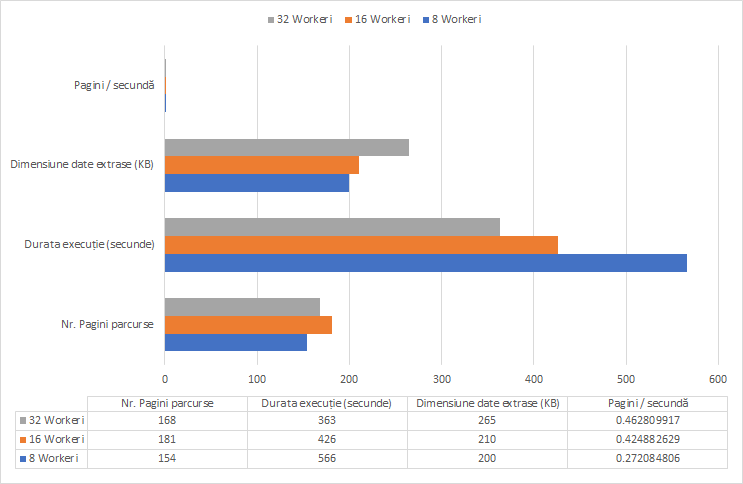
\includegraphics[keepaspectratio, scale=0.7]{depth-performance-chart.png}
	\end{adjustbox}
\end{center}
\end{figure}

\begin{figure}[ht]
\begin{center}
	\begin{adjustbox}{addcode={\begin{minipage}{\width}}{\caption{%
	      Performanța crawler-ului "Surf" la parcurgerile pe niveluri \cite{diagram-icons-sources, aws-icons-source, microsoft-excel}
	      }\end{minipage}},rotate=90,center}
	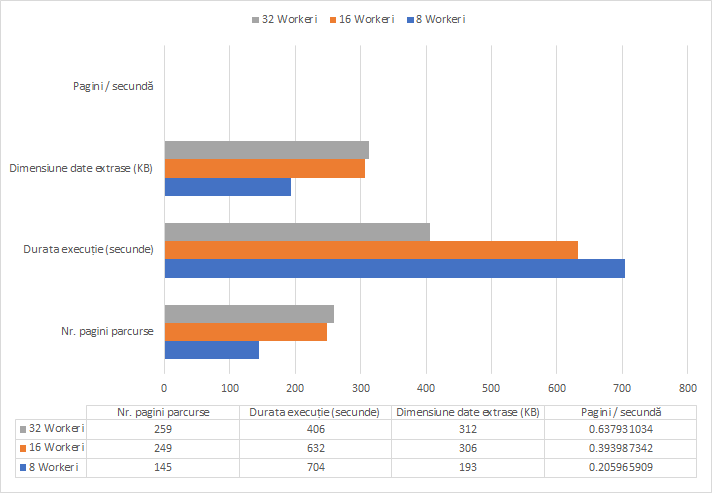
\includegraphics[keepaspectratio, scale=0.7]{breadth-performance-chart.png}
	\end{adjustbox}
\end{center}
\end{figure}

